\chapter{Harmonic, Damped, and Driven Oscillations}
\label{ch:oscillations}
\begin{chapterintro}
\textbf{You will learn to:} solve the differential equations of free, damped, and forced harmonic oscillators; analyze underdamped, critically damped, and overdamped regimes; determine the quality factor $Q$ and logarithmic decrement; calculate resonance frequency, amplitude, and phase lag; and study energy dissipation and resonance bandwidth.
\end{chapterintro}

\section{The Simple Harmonic Oscillator}

The ideal undamped harmonic oscillator obeys the linear differential equation:
\[
\boxed{\ddot{x} + \omega_0^2\,x = 0,}
\]
where $\omega_0 = \sqrt{k/m}$ is the \textbf{natural angular frequency}.
The general solution can be written in equivalent forms:
\[
\boxed{x(t) = A\cos(\omega_0 t + \phi) = C_1\cos(\omega_0 t) + C_2\sin(\omega_0 t) = \operatorname{Re}\left( \tilde{X} e^{\mathrm{i}\omega_0 t} \right),}
\]
where $A$ is the amplitude and $\phi$ is the initial phase determined by initial conditions:
\[
A = \sqrt{x_0^2 + \left(\frac{v_0}{\omega_0}\right)^2}, \qquad \tan\phi = -\frac{v_0}{\omega_0 x_0}.
\]
The period and frequency are:
\[
T_0 = \frac{2\pi}{\omega_0} = 2\pi\sqrt{\frac{m}{k}}, \qquad f_0 = \frac{1}{T_0} = \frac{\omega_0}{2\pi}.
\]

\begin{figure}[htbp]
\centering
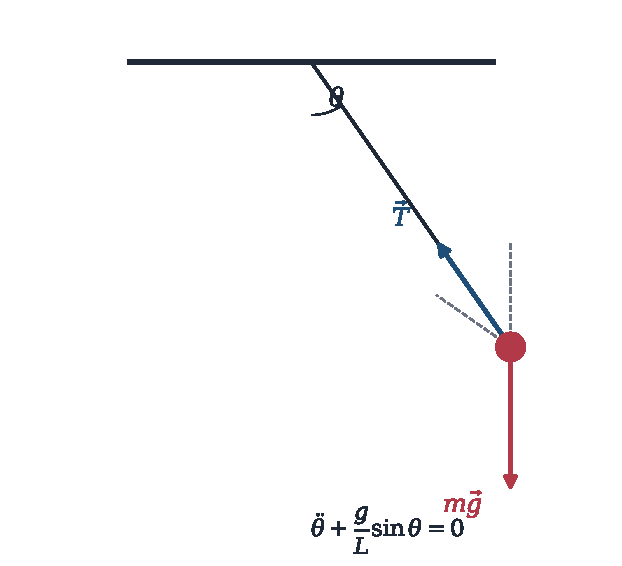
\includegraphics[width=0.48\textwidth]{figures/20_pendulum.pdf}
\caption{The simple pendulum of length $L$ oscillating at angle $\theta$ from the vertical. For small angles $\theta \ll 1$, it executes simple harmonic motion with natural frequency $\omega_0 = \sqrt{g/L}$.}
\label{fig:pendulum}
\end{figure}
The total mechanical energy is conserved:
\[
\boxed{E_m = \frac{1}{2}m v^2 + \frac{1}{2}k x^2 = \frac{1}{2}k A^2 = \frac{1}{2}m\omega_0^2 A^2 = \text{constant}.}
\]
Over one complete cycle, kinetic and potential energies share the total energy equally on average:
\[
\langle E_c \rangle = \langle E_p \rangle = \frac{1}{2}E_m.
\]

\begin{figure}[htbp]
\centering
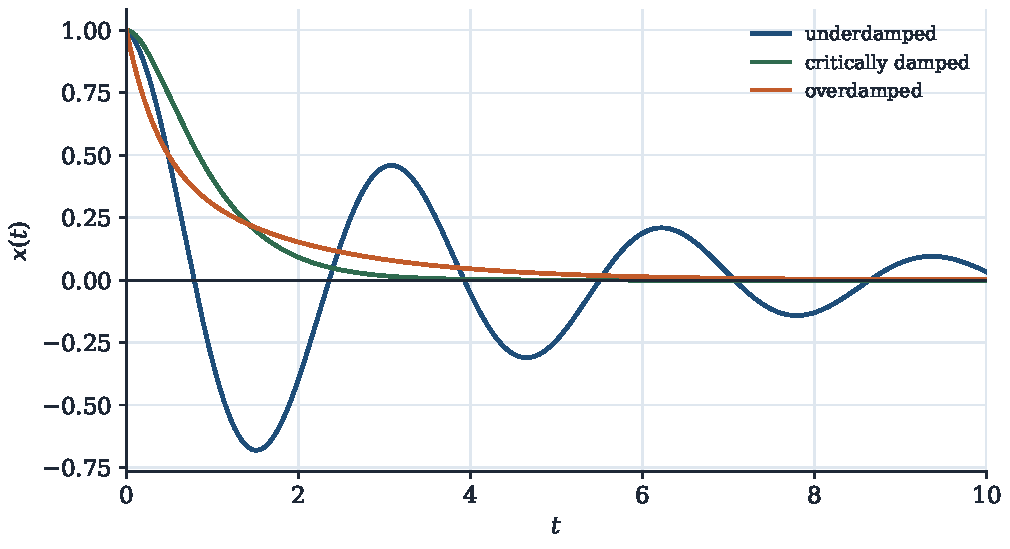
\includegraphics[width=0.74\textwidth]{figures/16_damped_oscillations.pdf}
\caption{Free damped oscillations in the underdamped regime ($\lambda < \omega_0$). The displacement decays within an exponential envelope $\pm A_0 e^{-\lambda t}$.}
\label{fig:damped_oscillations}
\end{figure}

\section{Damped Harmonic Oscillations}

When a viscous damping force $\vec{f} = -b\vec{v} = -b\dot{x}\ihat$ ($b > 0$) opposes motion, Newton's second law gives:
\[
m\ddot{x} + b\dot{x} + kx = 0 \implies \boxed{\ddot{x} + 2\lambda\dot{x} + \omega_0^2\,x = 0,}
\]
where $\lambda = \frac{b}{2m}$ is the \textbf{damping parameter}.
The characteristic equation is $r^2 + 2\lambda r + \omega_0^2 = 0$, with roots $r_{1, 2} = -\lambda \pm \sqrt{\lambda^2 - \omega_0^2}$.

Three distinct physical regimes arise depending on the discriminant $\Delta = \lambda^2 - \omega_0^2$:

\begin{center}
\renewcommand{\arraystretch}{1.3}
\begin{tabular}{@{}llll@{}}
\toprule
\textbf{Regime} & \textbf{Condition} & \textbf{General Solution $x(t)$} & \textbf{Physical Behavior} \\
\midrule
\textbf{Underdamped} & $\lambda < \omega_0$ & $A_0 e^{-\lambda t}\cos(\omega_d t + \phi)$ & Oscillations with decaying amplitude; $\omega_d = \sqrt{\omega_0^2 - \lambda^2}$ \\
\textbf{Critically Damped} & $\lambda = \omega_0$ & $(C_1 + C_2 t)e^{-\lambda t}$ & Fastest return to equilibrium without oscillating \\
\textbf{Overdamped} & $\lambda > \omega_0$ & $C_1 e^{r_1 t} + C_2 e^{r_2 t}$ & Sluggish non-oscillatory exponential return \\
\bottomrule
\end{tabular}
\end{center}

\begin{keyidea}[Key Parameters of Damped Systems]
\begin{itemize}[leftmargin=1.4em,itemsep=2pt]
  \item \textbf{Pseudo-period}: $T_d = \frac{2\pi}{\omega_d} = \frac{2\pi}{\sqrt{\omega_0^2 - \lambda^2}} > T_0$.
  \item \textbf{Logarithmic decrement}: The natural logarithm of the ratio of two successive peak displacements separated by one period $T_d$:
        \[
        \boxed{\delta = \ln\left(\frac{x(t)}{x(t + T_d)}\right) = \lambda T_d = \frac{2\pi\lambda}{\omega_d}.}
        \]
  \item \textbf{Quality factor $Q$}: Dimensionless figure of merit measuring sharpness of resonance and low dissipation:
        \[
        \boxed{Q = \frac{\omega_0}{2\lambda} = \frac{m\omega_0}{b} \approx \frac{\pi}{\delta}.}
        \]
        In one cycle, the fractional energy lost is $\frac{\Delta E_m}{E_m} \approx \frac{2\pi}{Q}$.
\end{itemize}
\end{keyidea}

\section{Driven (Forced) Oscillations and Resonance}

Apply an external sinusoidal driving force $F(t) = F_0\cos(\omega t)$:
\[
\boxed{\ddot{x} + 2\lambda\dot{x} + \omega_0^2\,x = \frac{F_0}{m}\cos(\omega t).}
\]
After transients die out, the \textbf{steady-state response} is sinusoidal at the driving frequency $\omega$:
\[
\boxed{x_p(t) = X(\omega)\cos(\omega t - \phi),}
\]
where the steady-state amplitude $X(\omega)$ and phase lag $\phi(\omega)$ are:
\[
\boxed{X(\omega) = \frac{F_0/m}{\sqrt{(\omega_0^2 - \omega^2)^2 + 4\lambda^2\omega^2}},} \qquad \boxed{\tan\phi(\omega) = \frac{2\lambda\omega}{\omega_0^2 - \omega^2}.}
\]

\begin{keyidea}[Resonance Phenomena]
\begin{itemize}[leftmargin=1.4em,itemsep=2pt]
  \item \textbf{Amplitude Resonance}: The amplitude $X(\omega)$ reaches its maximum at the \textbf{resonance frequency}:
        \[
        \boxed{\omega_{\text{res}} = \sqrt{\omega_0^2 - 2\lambda^2} = \omega_0\sqrt{1 - \frac{1}{2Q^2}}.}
        \]
        (Resonance occurs only if $\lambda < \omega_0/\sqrt{2}$, i.e., $Q > 1/\sqrt{2}$).
  \item \textbf{Peak Amplitude}: At $\omega = \omega_{\text{res}}$:
        \[
        X_{\max} = \frac{F_0/m}{2\lambda\sqrt{\omega_0^2 - \lambda^2}} \approx Q\left(\frac{F_0}{k}\right) \quad (\text{for } Q \gg 1).
        \]
        The static deflection $x_{\text{static}} = F_0/k$ is magnified by a factor of $Q$!
  \item \textbf{Velocity Resonance}: The velocity amplitude is maximized exactly at $\omega = \omega_0$, where the response is in \textbf{quadrature} ($\phi = \pi/2$), meaning the driving force is always in phase with velocity ($P(t) \ge 0$).
  \item \textbf{Resonance Bandwidth}: The width between half-power points ($\Delta\omega = \omega_2 - \omega_1$) satisfies:
        \[
        \boxed{\Delta\omega = 2\lambda = \frac{\omega_0}{Q}.}
        \]
\end{itemize}
\end{keyidea}

\section{Worked Examples}

\begin{worked}[Determining damping and $Q$ from an oscilloscope trace]
An underdamped mechanical oscillator of mass $m=0.100\ \mathrm{kg}$ has a natural frequency $f_0 = 5.00\ \mathrm{Hz}$. Its recorded amplitude drops from $x_0 = 4.00\ \mathrm{cm}$ to $x_{10} = 1.00\ \mathrm{cm}$ after $N = 10$ full oscillations.
Find the logarithmic decrement $\delta$, the damping constant $\lambda$, the quality factor $Q$, and the damping coefficient $b$.
\end{worked}

\begin{solution}{15.1}
The amplitude after $N$ cycles decays according to $x_N = x_0 e^{-N\lambda T_d}$:
\[
\frac{x_0}{x_N} = e^{N\lambda T_d} = e^{N\delta} \implies N\delta = \ln\left(\frac{x_0}{x_N}\right).
\]
For $N = 10$ and $x_0/x_{10} = 4.00/1.00 = 4.00$:
\[
10\delta = \ln(4.00) = 1.3863 \implies \boxed{\delta = \frac{1.3863}{10} \approx \mathbf{0.1386.}}
\]
Since $\delta \ll 1$, damping is weak, so $\omega_d \approx \omega_0$:
\[
T_d \approx T_0 = \frac{1}{f_0} = \frac{1}{5.00} = 0.200\ \mathrm{s}.
\]
The damping parameter is:
\[
\lambda = \frac{\delta}{T_d} = \frac{0.1386}{0.200} = \mathbf{0.693\ \mathrm{s^{-1}}.}
\]
The quality factor is:
\[
Q = \frac{\pi}{\delta} = \frac{\pi}{0.1386} \approx \mathbf{22.7.}
\]
The viscous damping coefficient is:
\[
b = 2m\lambda = 2(0.100\ \mathrm{kg})(0.693\ \mathrm{s^{-1}}) = \mathbf{0.139\ \mathrm{kg\,s^{-1}}.}
\]
\end{solution}

\begin{worked}[Driven oscillator at resonance]
A spring-mass system with $m = 0.500\ \mathrm{kg}$, $k = 200\ \mathrm{N\,m^{-1}}$, and $b = 0.800\ \mathrm{kg\,s^{-1}}$ is driven by an external force $F(t) = F_0\cos(\omega t)$ with $F_0 = 4.00\ \mathrm{N}$.
(a) Find the natural angular frequency $\omega_0$, damping factor $\lambda$, and quality factor $Q$.
(b) Find the resonance frequency $\omega_{\text{res}}$ and the amplitude at resonance $X_{\max}$.
(c) Compute the average power supplied by the driver at velocity resonance ($\omega = \omega_0$).
\end{worked}

\begin{solution}{15.2}
(a) Fundamental parameters:
\[
\omega_0 = \sqrt{\frac{k}{m}} = \sqrt{\frac{200}{0.500}} = \mathbf{20.0\ \mathrm{rad\,s^{-1}}.}
\]
\[
\lambda = \frac{b}{2m} = \frac{0.800}{2(0.500)} = \mathbf{0.800\ \mathrm{s^{-1}}.}
\]
\[
Q = \frac{\omega_0}{2\lambda} = \frac{20.0}{2(0.800)} = \mathbf{12.5.}
\]

(b) Resonance frequency:
\[
\omega_{\text{res}} = \sqrt{\omega_0^2 - 2\lambda^2} = \sqrt{20.0^2 - 2(0.800)^2} = \sqrt{400 - 1.28} = \sqrt{398.72} \approx \mathbf{19.97\ \mathrm{rad\,s^{-1}}.}
\]
The amplitude at resonance is:
\[
X_{\max} = \frac{F_0/m}{2\lambda\sqrt{\omega_0^2 - \lambda^2}} = \frac{4.00/0.500}{2(0.800)\sqrt{400 - 0.64}} = \frac{8.00}{1.60\times 19.98} = \frac{8.00}{31.97} \approx \mathbf{0.250\ \mathrm{m}} = 25.0\ \mathrm{cm}.
\]
Notice that static deflection is $x_{\text{st}} = F_0/k = 4.00/200 = 0.020\ \mathrm{m} = 2.0\ \mathrm{cm}$. The resonance magnifies the motion by a factor of $X_{\max}/x_{\text{st}} = 25.0/2.0 = 12.5 = Q$!

(c) At $\omega = \omega_0 = 20.0\ \mathrm{rad\,s^{-1}}$, the force and velocity are in phase ($\phi = \pi/2$). The velocity amplitude is $V_0 = \omega_0 X(\omega_0) = \frac{F_0}{b}$:
\[
V_0 = \frac{4.00}{0.800} = 5.00\ \mathrm{m\,s^{-1}}.
\]
The average power supplied by the driver (which equals the power dissipated by friction) is:
\[
\langle P \rangle = \frac{1}{2}F_0 V_0 = \frac{1}{2}(4.00\ \mathrm{N})(5.00\ \mathrm{m\,s^{-1}}) = \mathbf{10.0\ \mathrm{W}.}
\]
\end{solution}

\section{Exercises and Step-by-Step Solutions}

\begin{exercise}{\warm\ General solution from initial conditions}
A horizontal spring-mass oscillator has mass $m=0.200\ \mathrm{kg}$ and spring stiffness $k=80.0\ \mathrm{N\,m^{-1}}$. At $t=0$, the mass is displaced to $x_0 = +5.00\ \mathrm{cm} = 0.0500\ \mathrm{m}$ and given an initial velocity $v_0 = -0.600\ \mathrm{m\,s^{-1}}$ directed toward the origin.
(a) Find the natural angular frequency $\omega_0$ and the period $T_0$.
(b) Write the position $x(t) = A\cos(\omega_0 t + \phi)$, finding $A$ and $\phi$.
(c) Calculate the total mechanical energy $E_m$.
\end{exercise}

\begin{tabletworkspace}[5.0cm]
\end{tabletworkspace}

\begin{solution}{15.1}
(a) Angular frequency:
\[
\omega_0 = \sqrt{\frac{k}{m}} = \sqrt{\frac{80.0}{0.200}} = \sqrt{400} = \mathbf{20.0\ \mathrm{rad\,s^{-1}}.}
\]
Period:
\[
T_0 = \frac{2\pi}{\omega_0} = \frac{2\pi}{20.0} = \frac{\pi}{10} \approx \mathbf{0.314\ \mathrm{s}.}
\]

(b) Amplitude:
\[
A = \sqrt{x_0^2 + \left(\frac{v_0}{\omega_0}\right)^2} = \sqrt{(0.0500)^2 + \left(\frac{-0.600}{20.0}\right)^2} = \sqrt{0.00250 + (-0.0300)^2} = \sqrt{0.00250 + 0.00090} = \sqrt{0.00340} \approx \mathbf{0.0583\ \mathrm{m}} = 5.83\ \mathrm{cm}.
\]
Phase angle $\phi$:
\[
\tan\phi = -\frac{v_0}{\omega_0 x_0} = -\frac{-0.600}{20.0\times 0.0500} = +\frac{0.600}{1.000} = +0.600.
\]
Since $x_0 > 0$ and $\cos\phi = x_0/A > 0$, $\phi$ is in the first quadrant:
\[
\phi = \arctan(0.600) \approx 0.540\ \mathrm{rad} \approx 31.0^\circ.
\]
The full trajectory is:
\[
\boxed{x(t) = 0.0583\cos(20.0 t + 0.540)\ \mathrm{m}.}
\]

(c) Mechanical energy:
\[
E_m = \frac{1}{2}k A^2 = \frac{1}{2}(80.0)(0.0583)^2 = 40.0\times 0.00340 = \mathbf{0.136\ \mathrm{J}.}
\]
Check with initial values: $E_m = \frac{1}{2}k x_0^2 + \frac{1}{2}m v_0^2 = \frac{1}{2}(80.0)(0.05)^2 + \frac{1}{2}(0.20)(-0.6)^2 = 0.100 + 0.036 = 0.136\ \mathrm{J}$ (exact agreement!).
\end{solution}

\begin{exercise}{\warm\ The Virial Theorem for harmonic oscillations}
For an undamped harmonic oscillator $x(t) = A\cos(\omega_0 t + \phi)$:
(a) Write the instantaneous kinetic energy $E_c(t)$ and potential energy $E_p(t)$.
(b) Calculate the time-average of both energies over one complete period $T_0$:
\[
\langle E_c \rangle = \frac{1}{T_0}\int_0^{T_0} E_c(t)\dd t, \qquad \langle E_p \rangle = \frac{1}{T_0}\int_0^{T_0} E_p(t)\dd t.
\]
(c) Verify that $\langle E_c \rangle = \langle E_p \rangle = \frac{1}{2}E_m$.
\end{exercise}

\begin{tabletworkspace}[5.0cm]
\end{tabletworkspace}

\begin{solution}{15.2}
(a) The position and velocity are:
\[
x(t) = A\cos(\omega_0 t + \phi), \qquad v(t) = \dot{x}(t) = -\omega_0 A\sin(\omega_0 t + \phi).
\]
Instantaneous energies:
\begin{align*}
E_p(t) &= \frac{1}{2}k x^2(t) = \frac{1}{2}k A^2\cos^2(\omega_0 t + \phi), \\
E_c(t) &= \frac{1}{2}m v^2(t) = \frac{1}{2}m\omega_0^2 A^2\sin^2(\omega_0 t + \phi) = \frac{1}{2}k A^2\sin^2(\omega_0 t + \phi).
\end{align*}

(b) Using the standard trigonometric integral averages:
\[
\frac{1}{T_0}\int_0^{T_0} \cos^2(\omega_0 t + \phi)\dd t = \frac{1}{2}, \qquad \frac{1}{T_0}\int_0^{T_0} \sin^2(\omega_0 t + \phi)\dd t = \frac{1}{2}.
\]
Therefore:
\begin{align*}
\langle E_p \rangle &= \frac{1}{2}k A^2\left(\frac{1}{2}\right) = \mathbf{\frac{1}{4}k A^2,} \\
\langle E_c \rangle &= \frac{1}{2}k A^2\left(\frac{1}{2}\right) = \mathbf{\frac{1}{4}k A^2.}
\end{align*}

(c) The total energy is $E_m = \frac{1}{2}k A^2$.
Comparing:
\[
\boxed{\langle E_c \rangle = \langle E_p \rangle = \frac{1}{2}E_m.}
\]
This equipartition of energy on average between kinetic and potential forms is a fundamental instance of the Virial Theorem for quadratic potentials ($V \propto r^2 \implies 2\langle E_c \rangle = 2\langle E_p \rangle$).
\end{solution}

\begin{exercise}{\core\ Critical damping for an automobile suspension}
A car wheel and suspension can be modeled as a quarter-car of mass $m=350\ \mathrm{kg}$ supported by a spring of stiffness $k=35.0\ \mathrm{kN\,m^{-1}} = 35000\ \mathrm{N\,m^{-1}}$ and a shock absorber (dashpot) of damping coefficient $b$.
(a) Find the natural angular frequency $\omega_0$ and the undamped oscillation frequency $f_0$.
(b) Calculate the critical damping coefficient $b_{\text{crit}}$ required for the suspension to return to equilibrium as quickly as possible without bouncing.
(c) If the shock absorber wears out and its damping drops to $b = 0.25\,b_{\text{crit}}$, find the pseudo-period $T_d$ and the fraction of amplitude remaining after one bounce.
\end{exercise}

\begin{tabletworkspace}[5.5cm]
\end{tabletworkspace}

\begin{solution}{15.3}
(a) Natural angular frequency:
\[
\omega_0 = \sqrt{\frac{k}{m}} = \sqrt{\frac{35000}{350}} = \sqrt{100} = \mathbf{10.0\ \mathrm{rad\,s^{-1}}.}
\]
Frequency:
\[
f_0 = \frac{\omega_0}{2\pi} = \frac{10.0}{2\pi} \approx \mathbf{1.59\ \mathrm{Hz}.}
\]

(b) Critical damping occurs when $\lambda = \omega_0$:
\[
\frac{b_{\text{crit}}}{2m} = \omega_0 \implies \boxed{b_{\text{crit}} = 2m\omega_0 = 2\sqrt{km}.}
\]
Computing:
\[
b_{\text{crit}} = 2(350)(10.0) = \mathbf{7000\ \mathrm{N\,s\,m^{-1}}} = 7.00\times 10^3\ \mathrm{kg\,s^{-1}}.
\]

(c) Worn shock absorber: $b = 0.25\,b_{\text{crit}} \implies \lambda = 0.25\,\omega_0 = 2.50\ \mathrm{s^{-1}}$.
The pseudo-frequency is:
\[
\omega_d = \sqrt{\omega_0^2 - \lambda^2} = \sqrt{10.0^2 - 2.5^2} = \sqrt{100 - 6.25} = \sqrt{93.75} \approx 9.68\ \mathrm{rad\,s^{-1}}.
\]
The pseudo-period is:
\[
T_d = \frac{2\pi}{\omega_d} = \frac{2\pi}{9.68} \approx \mathbf{0.649\ \mathrm{s}.}
\]
The decay per period is given by the factor $e^{-\lambda T_d}$:
\[
\lambda T_d = (2.50)(0.649) \approx 1.623 \implies \frac{A(t + T_d)}{A(t)} = e^{-1.623} \approx \mathbf{0.197} \approx 19.7\%.
\]
The car will noticeably bounce after hitting a pothole, retaining nearly $20\%$ of its displacement on the rebound!
\end{solution}

\begin{exercise}{\core\ Oscillations in a U-tube manometer}
A uniform glass U-tube of internal cross-sectional area $S$ contains a column of liquid of density $\rho$ and total column length $L$. The liquid is displaced by a distance $z_0$ in one arm and released.
(a) Neglecting viscosity, show that the column executes simple harmonic motion with equation:
\[
\ddot{z} + \frac{2g}{L}z = 0.
\]
(b) Find the period of oscillation $T$. Compare it with a simple pendulum.
(c) Liquid viscosity introduces a Poiseuille laminar drag force $F_d = -8\pi\eta L\dot{z}$, where $\eta$ is the dynamic viscosity. Write the damped differential equation and determine the condition on $\eta$ for the motion to remain underdamped.
\end{exercise}

\begin{tabletworkspace}[6.0cm]
\end{tabletworkspace}

\begin{solution}{15.4}
(a) The total mass of the liquid column is $m = \rho S L$.
When the liquid level rises by $z$ in the right arm, it drops by $z$ in the left arm.
The height difference between the two columns is $2z$.
The unbalanced weight of this excess column provides the restoring force:
\[
F_{\text{rest}} = -(\text{mass of excess column})g = -(\rho S\cdot 2z)g = -2\rho g S z.
\]
Applying Newton's second law $m\ddot{z} = F_{\text{rest}}$:
\[
(\rho S L)\ddot{z} = -2\rho g S z \implies \rho S L\ddot{z} + 2\rho g S z = 0.
\]
Dividing by $\rho S L$:
\[
\boxed{\ddot{z} + \frac{2g}{L}z = 0.}
\]

(b) The natural angular frequency is $\omega_0 = \sqrt{\frac{2g}{L}}$.
The period of oscillation is:
\[
\boxed{T = 2\pi\sqrt{\frac{L}{2g}}.}
\]
This is identical to the period of a simple pendulum of length $L_{\text{eff}} = \frac{L}{2}$!

(c) Adding the laminar viscous friction force $F_d = -b\dot{z}$ with $b = 8\pi\eta L$:
\[
m\ddot{z} + b\dot{z} + (2\rho g S)z = 0 \implies \ddot{z} + \frac{8\pi\eta}{\rho S}\dot{z} + \frac{2g}{L}z = 0.
\]
The damping parameter is $\lambda = \frac{b}{2m} = \frac{8\pi\eta L}{2\rho S L} = \frac{4\pi\eta}{\rho S}$.
For the motion to remain \textbf{underdamped} ($\lambda < \omega_0$):
\[
\frac{4\pi\eta}{\rho S} < \sqrt{\frac{2g}{L}} \implies \boxed{\eta < \frac{\rho S}{4\pi}\sqrt{\frac{2g}{L}}.}
\]
\end{solution}

\begin{exercise}{\mastery\ Two coupled oscillators and normal modes}
Two identical carts, each of mass $m$, can move along a frictionless horizontal track. Each cart is connected to a rigid wall by a spring of stiffness $k$, and the two carts are coupled to each other by a central spring of stiffness $k_c$.
(a) Write Newton's second law for displacements $x_1(t)$ and $x_2(t)$ from equilibrium.
(b) Define the \textbf{normal coordinates} $u(t) = x_1 + x_2$ (symmetric mode) and $v(t) = x_1 - x_2$ (antisymmetric mode). Show that they decouple into two independent harmonic oscillators.
(c) Find the two normal frequencies $\omega_1$ and $\omega_2$, and describe the physical motion in each mode.
\end{exercise}

\begin{tabletworkspace}[6.5cm]
\end{tabletworkspace}

\begin{solution}{15.5}
(a) The forces on each cart are:
\begin{align*}
m\ddot{x}_1 &= -kx_1 + k_c(x_2 - x_1) = -(k + k_c)x_1 + k_c x_2, \\
m\ddot{x}_2 &= -kx_2 - k_c(x_2 - x_1) = k_c x_1 - (k + k_c)x_2.
\end{align*}

(b) Adding the two equations:
\[
m(\ddot{x}_1 + \ddot{x}_2) = -k(x_1 + x_2) \implies m\ddot{u} + k u = 0 \implies \boxed{\ddot{u} + \omega_1^2 u = 0,}
\]
where $\omega_1 = \sqrt{\frac{k}{m}}$.

Subtracting the two equations:
\[
m(\ddot{x}_1 - \ddot{x}_2) = -(k + 2k_c)(x_1 - x_2) \implies m\ddot{v} + (k + 2k_c)v = 0 \implies \boxed{\ddot{v} + \omega_2^2 v = 0,}
\]
where $\omega_2 = \sqrt{\frac{k + 2k_c}{m}}$.
The normal coordinates $u(t)$ and $v(t)$ are completely decoupled!

(c) Physical description of the normal modes:
\begin{itemize}[leftmargin=1.4em,itemsep=2pt]
  \item \textbf{Mode 1 (Symmetric / In-phase)}: $v = 0 \implies x_1(t) = x_2(t)$.
  Frequency: $\boxed{\omega_1 = \sqrt{\frac{k}{m}}}$.
  Both carts move synchronously in the same direction with identical amplitude. The coupling spring maintains constant length ($x_2 - x_1 = 0$) and exerts no force; the carts oscillate as if the central spring did not exist!
  \item \textbf{Mode 2 (Antisymmetric / Out-of-phase)}: $u = 0 \implies x_1(t) = -x_2(t)$.
  Frequency: $\boxed{\omega_2 = \sqrt{\frac{k + 2k_c}{m}}}$.
  The carts move in opposite directions, alternately compressing and expanding the central spring. The restoring force is stronger, so $\omega_2 > \omega_1$.
\end{itemize}
Any general motion is a linear superposition $x_1(t) = \frac{1}{2}(u(t) + v(t))$ and $x_2(t) = \frac{1}{2}(u(t) - v(t))$, giving rise to the phenomenon of \textbf{beats} when $k_c \ll k$.
\end{solution}
